\thispagestyle{empty}
\chapter{Vuelo en Espiral}

\spacing{1.5}

Igual que se ha hecho en el capítulo anterior con el vuelo horizontal, este capítulo pretende abordar el estado del helicóptero durante un vuelo en espiral ascendente con ángulo de asiento de la velocidad $\gamma_T$=5$^\circ$, giro a la derecha y un radio de giro de la trayectoria de 150 m.
Lo primero que salta a la vista en la gráfica \ref{PMVE} es la reducción de la velocidad de avance máxima a la que se puede volar, siendo esta 42.37 m/s, lo que supone una reducción de casi 30 m/s respecto al vuelo horizontal, lo que se debe a la necesidad de invertir una parte importante de la potencia en conseguir una velocidad vertical. Dicha velocidad vertical se ha representado en la gráfica \ref{VzVE}. Al ser el ángulo de asiento de la velocidad constante, la velocidad de ascenso varía de forma casi lineal con la velocidad de avance.

\begin{figure}
	\centering
	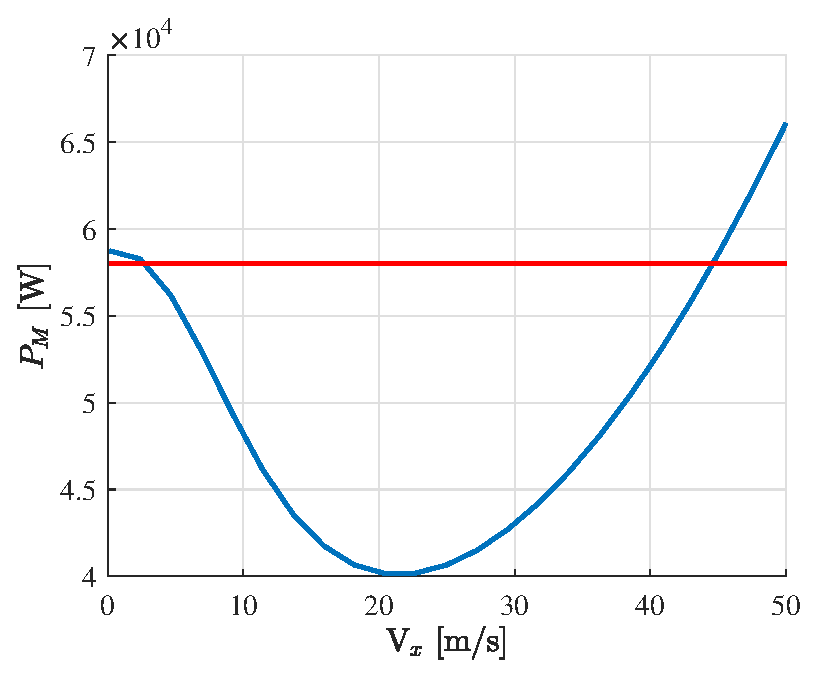
\includegraphics[width=90mm]{graficos/PMVE}
	\caption{Consumo de Potencia de la aeronave en función de la velocidad de avance a nivel del mar para vuelo en espiral ascendente con $\gamma_T$=5$^\circ$, giro a la derecha y radio de la trayectoria 150 m. La línea roja representa el valor de la potencia máxima continua que puede proporcionar el motor.}
	\label{PMVE}
\end{figure}
\begin{figure}
	\centering
	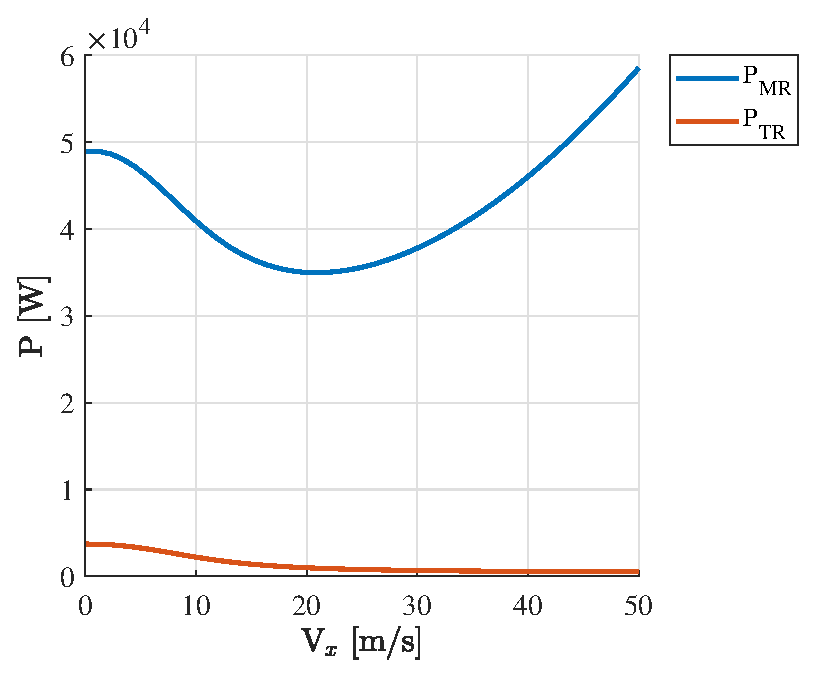
\includegraphics[width=90mm]{graficos/PVE}
	\caption{Consumo de Potencia de los rotores principal y antipar en función de la velocidad de avance a nivel del mar para vuelo en espiral ascendente con $\gamma_T$=5$^\circ$, giro a la derecha y radio de la trayectoria 150 m.}
	\label{PVE}
\end{figure}
\begin{figure}
	\centering
	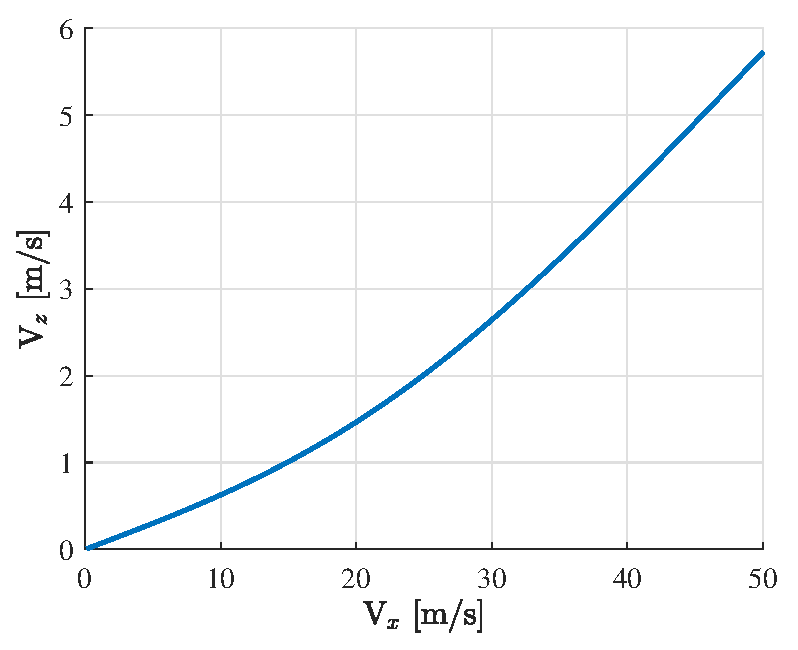
\includegraphics[width=90mm]{graficos/VzVE}
	\caption{Velocidad vertical de la aeronave en función de la velocidad de avance a nivel del mar para vuelo en espiral ascendente con $\gamma_T$=5$^\circ$, giro a la derecha y radio de la trayectoria 150 m.}
	\label{VzVE}
\end{figure}
\begin{figure}
	\centering
	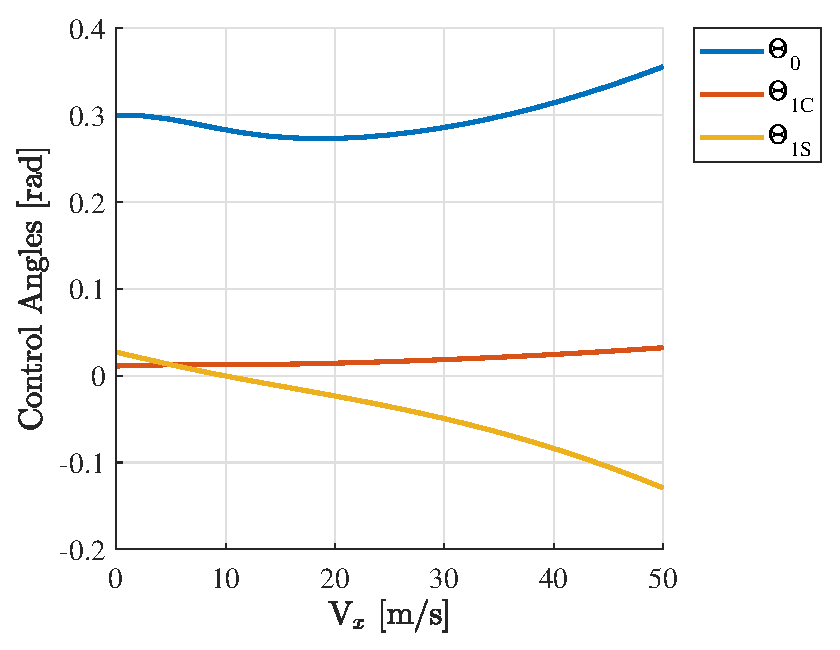
\includegraphics[width=90mm]{graficos/ControlVE}
	\caption{Ángulos de control de la aeronave en función de la velocidad de avance a nivel del mar para vuelo en espiral ascendente con $\gamma_T$=5$^\circ$, giro a la derecha y radio de la trayectoria 150 m.}
	\label{ControlVE}
\end{figure}

Los ángulos de control se han reflejado en gráfica \ref{ControlVE}, y si la comparamos con la gráfica \ref{ControlVH} del vuelo horizontal se puede apreciar que mientras el ángulo de paso cíclico lateral $\theta_{1C}$ sigue una evolución similar, el ángulo de paso colectivo $\theta_0$ aumenta de forma significativa. Esto se debe al incremento de sustentación necesario para poder elevar la aeronave. Por otra parte, se ve como el ángulo de paso longitudinal $\theta_{1S}$ disminuye, ya que la sustentación ha de tener una mayor componente vertical para no solo compensar el peso de la aeronave sino poder elevarla a su vez.

\begin{figure}
	\centering
	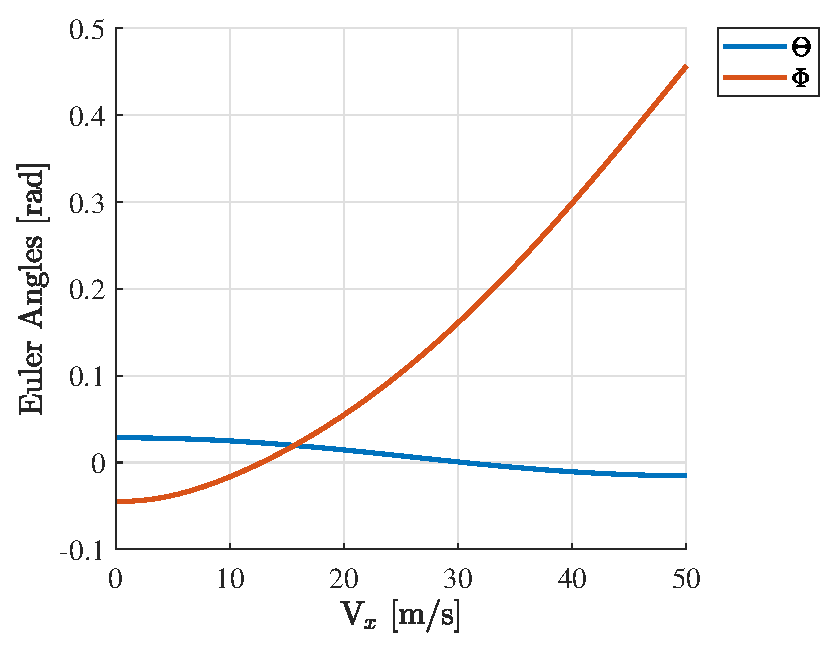
\includegraphics[width=90mm]{graficos/EulerVE}
	\caption{Ángulos de Euler de la aeronave en función de la velocidad de avance a nivel del mar para vuelo en espiral ascendente con $\gamma_T$=5$^\circ$, giro a la derecha y radio de la trayectoria 150 m.}
	\label{EulerVE}
\end{figure}

En lo que respecta a los ángulos de Euler, el cambio también resulta lógico. En la gráfica \ref{EulerVH} del capítulo anterior se observa que con la velocidad, apenas cambia el balanceo, mientras que el cabeceo disminuye, pero en la gráfica \ref{EulerVE} par el vuelo en espiral ocurre algo muy distinto.
El ángulo de cabeceo apenas apenas cambia mientras que el ángulo de balanceo aumenta con la velocidad. Si se mantiene constante la curvatura de la espiral, según aumenta la velocidad de avance la aceleración normal necesaria para mantener la trayectoria aumenta, de ahí el origen de ese incremento en el ángulo de balanceo.

\section{Velocidad de Ascenso del Vuelo}

A diferencia del caso del vuelo horizontal, donde interesaba conocer la autonomía del helicóptero, este tipo de vuelo no será el principal de la aeronave, por lo que en ningún caso el vehículo volará en estas circunstancias durante una fracción relevante de su tiempo de vuelo. Otro parámetro típico que podría calcularse en este tipo de vuelos es el techo de la aeronave, pero como UAV de vigilancia, no interesará que realice vuelos a altitudes muy elevadas pues podría interferir en su misión por no ser las cámaras equipadas capaces de captar imágenes nítidas en esas condiciones.
Sin embargo, si podría resultar interesante observar como varía el vuelo con la velocidad vertical. Para ello se asume que el vehículo vuela con una velocidad de avance 
